%% Please change the file name by replacing N with the apporpriate number
%% corresponding to the current homework and XX with your initials.
%% https://www.math.uci.edu/~gpatrick/jsOnline/hw1.html

\documentclass{beamer}
\usepackage{amssymb,amsfonts,color,graphicx,amsmath,enumerate}
\usepackage{tikz} %This package offers the ability to draw pictures
\usepackage{amsthm}

\newcommand{\naturals}{\mathbb{N}}
\newcommand{\integers}{\mathbb{Z}}
\newcommand{\complex}{\mathbb{C}}
\newcommand{\reals}{\mathbb{R}}
\newcommand{\exreals}{\overline{\mathbb{R}}}
\newcommand{\mcal}[1]{\mathcal{#1}}
\newcommand{\mable}{measurable}
\newcommand{\quats}{\mathbb{H}}
\newcommand{\rationals}{\mathbb{Q}}
\newcommand{\norm}{\trianglelefteq}
\newcommand{\Aut}{\text{Aut}}
\newcommand{\disk}{\mathbb{D}}
\newcommand{\halfplane}{\mathbb{H}}
\newcommand{\Lp}[2]{\left\|{#1}\right\|_{L^{#2}}}
\newcommand{\supp}[1]{\text{supp}({#1})}
\newcommand{\Hom}[2]{\text{Hom}_{{#1}}({#2})}
\newcommand{\tr}{\text{tr}}
\newcommand{\field}[1]{\mathbb{F}_{{#1}}}
\newcommand{\Gal}[1]{\text{Gal}\left({#1}\right)}
\newcommand{\esssup}{\text{ess sup }}
\newcommand{\essinf}{\text{ess inf }}
\newcommand{\affine}{\mathbb{A}}

% \newenvironment{solution}
% {\begin{proof}[Solution]}
% {\end{proof}}

% \voffset=-3cm
% \hoffset=-2.25cm
% \textheight=24cm
% \textwidth=17.25cm
% \addtolength{\jot}{8pt}
% \linespread{1.3}

\title{Braid Group Cryptography}
\author{Liam Hardiman}

\usetheme{Frankfurt}


\begin{document}
\maketitle

\begin{frame}
	\frametitle{Finitely Presented Groups}
	A finitely presented group $G=\langle S | R\rangle$ is specified by two sets, $S = \{x_i\}_{i\in I}$ and $R = \{r_j\}_{j\in J}$.\pause
	\begin{itemize}
		\item $S$ is a set of symbols called \textbf{generators}.\pause
		\item $R$ is a set of words in $S$ called \textbf{relators}. A \textbf{word} in $S$ is a finite string consisting of symbols in $S$ and the symbols $x_i^{-1}$, where $x_i\in S$. The empty string, $e$, is also a word.\pause
		\item We form a group by taking all possible words in $S$. The inverse of a word $w$ is formed by writing the symbols in $w$ in reverse order and replacing each $x_j$ appearing in $w$ by $x_j^{-1}$. The group operation is concatenation of words.
	\end{itemize}
\end{frame}

\begin{frame}
	\frametitle{Finitely Presented Groups}
	We form $G$ from $S$ and $R$ by taking all equivalence classes of words in $S$. Two words $v$ and $w$ are equivalent if $v$ can be transformed into $w$ by a finite sequence of these operations.\pause
	\begin{enumerate}
		\item Replacing $x_ix_i^{-1}$ or $x_i^{-1}x_i$ with $e$\pause
		\item Inserting $x_ix_i^{-1}$ or $x_i^{-1}x_i$ at any position\pause
		\item Replacing $r_j$ with $e$\pause
		\item Inserting $r_j$ at any position\pause
	\end{enumerate}
	Equivalently, $G$ is the quotient of the free group on $S$ by the normal closure of $R$. We say $G$ is \textbf{finitely presented} if $S$ and $R$ are finite sets.
\end{frame}

\begin{frame}
	\frametitle{Finitely Presented Groups}
	Some examples of finitely presented groups include...\pause
	\begin{itemize}
		\item Finite groups\pause
		\item The free group $F_n$ on $n$ generators\pause
		\item Finitely generated abelian groups\pause
		\item The braid group $B_n$, $n\geq 0$.\pause
	\end{itemize}
	Nonexamples include\pause
	\begin{itemize}
		\item Any group with infinitely many generators, e.g. $\integers^{\oplus \integers}$\pause
		\item There are finitely generated groups that are not finitely related, e.g. the wreath product of $\integers$ with itself.
	\end{itemize}
\end{frame}

\begin{frame}
	\frametitle{The Word Problem}
	Say we have a finitely presented group $G$.\pause
	\begin{block}{The word problem in $G$}
		\begin{quote}
		\begin{itemize}
			\item[input: ]two words $v, w$ in the generators of $G$
			\item[output: ]\textbf{yes} if $v$ is equivalent to $w$. \textbf{no} otherwise
		\end{itemize}
		\end{quote}
	\end{block}\pause
	\begin{example}[The word problem in $F_2 = \langle a, b\rangle$]
		Iteratively scan through both words, deleting adjacent inverses.\\\pause
		Given $v = aa^{-1}bba$ and $w = babb^{-1}a^{-1}ba$, we have\pause
		\begin{align*}
			\color{red}aa^{-1}\color{black}bba &= bba\\
			b\color{red}a\color{blue}{bb^{-1}}\color{red}a^{-1}\color{black}ba &= bba.
		\end{align*}\pause
		Output \textbf{yes}.
	\end{example}
\end{frame}

\begin{frame}
	\frametitle{The Word Problem}
	In 1955 Pyotr Novikov showed that there are finitely presented groups in which the word problem is \textbf{undecidable} - it is provably impossible to construct an algorithm that always outputs the correct answer.
\end{frame}

\begin{frame}
	\frametitle{The Conjugacy Search Problem}
	Let $G$ be a group.\pause
	\begin{block}{The Conjugacy Search Problem in $G$}
		\begin{quote}
			\begin{itemize}
				\item[input: ]Two conjugate words $u$ and $v$ in the generators of $G$.
				\item[output: ]A word $w$ such that $u = w^{-1}vw = v^w$
			\end{itemize}
		\end{quote}
	\end{block}\pause
	This is analogous to the discrete logarithm problem in a finite abelian group $H$.\pause
	\begin{block}{Discrete Logarithm Problem in $H$}
		\begin{quote}
			\begin{itemize}
				\item[input: ]Elements $g,h$ of $H$ such that $h\in \langle g\rangle$
				\item[output: ]An integer $k$ such that $g^k = h$
			\end{itemize}
		\end{quote}
	\end{block}
\end{frame}

\begin{frame}
	\frametitle{The Braid Group}
	\begin{definition}
		The braid group on $n$ strands, $B_n$ is defined by the presentation
		\begin{multline*}
		B_n = \langle \sigma_1, \sigma_2, \ldots, \sigma_{n-1}\ |\ \sigma_i\sigma_j\sigma_i = \sigma_j\sigma_i\sigma_j,\ |i-j|=1;\\ \sigma_i\sigma_j = \sigma_j\sigma_i,\ |i-j|>1\rangle.
		\end{multline*}
	\end{definition}\pause
	There is, however, a more geometric understanding of the braid group.
\end{frame}

\begin{frame}
	\frametitle{The Braid Group}
	\begin{itemize}
	\item Arrange two sets of $n$ items in vertical columns on opposite sides of the page. Fasten one end of a string to each item on the left side of the page. To each item on the right side attach the other end of one string. This connection is a \textbf{braid}.\pause

	\item The generator $\sigma_i$ represents connecting the $i$-th item on the left to the $i+1$st on the right and the $i+1$st on the left to the $i$-th on the right with the latter string passing over the former.\pause

	\item Two connections that can be made to look the same by tightening the strings are considered the same braid.\pause

	\item Composing two braids consists of drawing them next to one another, gluing the points in the middle, and connecting the strands.
	\end{itemize}
\end{frame}

\begin{frame}
	\frametitle{The Braid Group}
	\begin{example}
		In $B_4$ the generators $\sigma_1$, $\sigma_2$, $\sigma_3$ can be represented by these braid diagrams.
	\end{example}\pause
	\vfill
	\centering
	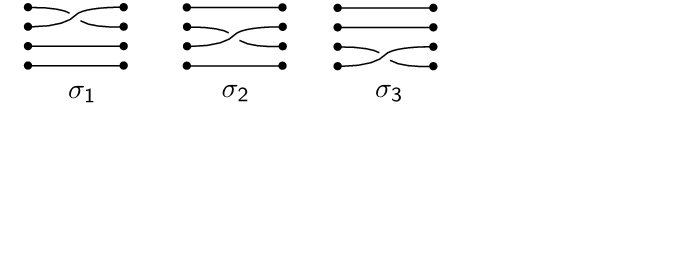
\includegraphics[scale=.7]{b4gens.png}
\end{frame}

\begin{frame}
	\frametitle{The Braid Group}
	\centering
	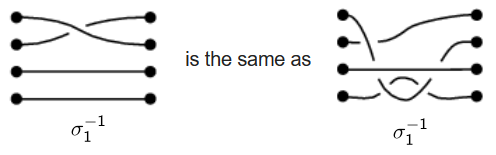
\includegraphics[scale=.6]{same.PNG}
\end{frame}

\begin{frame}
	\frametitle{The Braid Group}
	\begin{example}
		Here's an example of composition of braids in $B_4$.
	\end{example}\pause
	\vfill
	\centering
	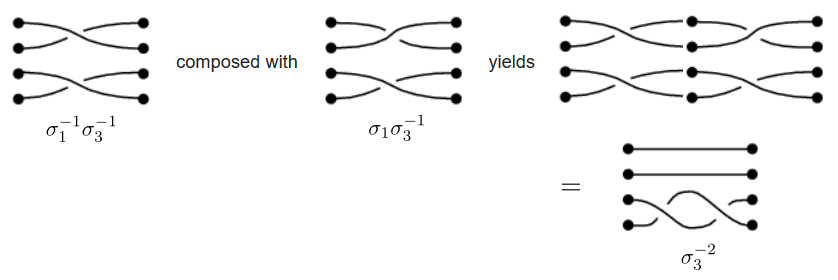
\includegraphics[scale=.5]{composition.png}
\end{frame}

\begin{frame}
	\frametitle{Braid Group Facts}
	\begin{itemize}
		\item $B_1$ is the trivial group. $B_2 \cong \integers$. $B_n$ for $n\geq 3$ is infinite and non-commutative.\pause
		\item The $n-1$ transpositions $(i, i+1)$ in the symmetric group $S_n$ obey the braid relations and generate $S_n$. Consequently, there is a surjective homomorphism $\rho: B_n\to S_n$ that sends $\sigma_i$ to $(i, i+1)$.
	\end{itemize}
\end{frame}

\begin{frame}
	\frametitle{Special Braids}
	\begin{definition}[Permutation Braid]
		To each permutation $\tau = b_1b_2\cdots b_n\in S_n$, associate an $n$-braid $A$ by connecting the right $i$-th point to the left $b_i$-th point with positive crossings (the strand from $i$ to $b_i$ passes under the one from $j$ to $b_j$ if $i<j$). A braid of this form is called a \textbf{permutation braid} or \textbf{canonical factor}. The set of all such braids is denoted $\tilde{\Sigma}_n$.
	\end{definition}\pause
	\vfill
	\begin{figure}[h]
		\centering
		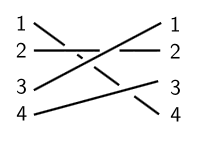
\includegraphics[scale=.7]{permutation.png}
		\caption{The braid $A\in \tilde{\Sigma}_4$ corresponding to $\pi = 4213\in S_4$.}
	\end{figure}
\end{frame}

\begin{frame}
	\frametitle{Special Braids}
	\begin{definition}[Fundamental Braid]
		The permutation braid corresponding to the permutation $\Omega_n = n(n-1)\cdots(2)1$ is called the \textbf{fundamental braid} and is denoted by $\Delta_n$.
	\end{definition}\pause
	\vfill
	\begin{figure}[h]
		\centering
		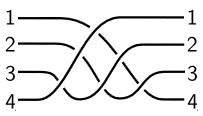
\includegraphics[scale=.7]{fundamental.png}
		\caption{The fundamental braid $\Delta_4\in B_4$ corresponding to the permutation $\Omega_4 = 4321$.}
	\end{figure}
\end{frame}

\begin{frame}
	\frametitle{Left-Canonical Form for Braids}
	\begin{theorem}[Elrifai and Morton '94]
		For any $W\in B_n$ there is a unique representation called the \textbf{left-canonical form} given by
		\[
		W = \Delta^uA_1A_2\cdots A_p,\quad u\in \integers, A_i\in \tilde{\Sigma}_n\setminus \{e, \Delta\},
		\]
		where $A_iA_{i+1}$ is left-weighted for $1\leq i\leq p-1$. We call $p$ the \textbf{canonical length} of $W$.
	\end{theorem}\pause
	Note that the correspondence between a permutation $\pi \in S_n$ to its canonical factor $A\in B_n$ is a right inverse of the homomorphism $\rho: B_n\to S_n$, so the cardinality of $\tilde{\Sigma}_n$ is $n!$. 
\end{frame}

\begin{frame}
	\frametitle{Left-Canonical Form for Braids}
	\begin{theorem}[Ko et al.\ 2000 using Epstein et al.\ '92]
	\begin{enumerate}
		\item Let $W$ be any word in $\sigma_1, \ldots, \sigma_n\in B_n$ with word length $\ell$. Then the left-canonical form of $W$ can be computed in time $O(\ell^2 n\log n)$.\pause
		\item Let $U = \Delta^uA_1\cdots A_p$ and $V = \Delta^vB_1\cdots B_q$ be the left-canonical forms of two $n$-braids. Then we can compute the left canonical form of $UV$ in time $O(pqn\log n)$.\pause
		\item If $U = \Delta^uA_1\cdots A_p$ is the left-canonical form of $U\in B_n$, then we can compute the left-canonical form of $U^{-1}$ in time $O(pn)$.\pause
	\end{enumerate}
	\end{theorem}
	These two theorems show that the word problem in $B_n$ is efficiently solvable, that is, we can efficiently differentiate between any two given elements of $B_n$.
\end{frame}


\begin{frame}
	\frametitle{Diffie-Hellman with Braids: Anshel, Anshel, Goldfeld '99}
	\begin{enumerate}
		\item Alice and Bob publicly agree on subgroups $B_n$, $A = \langle a_1, \ldots, a_k\rangle$ and $B = \langle b_1, \ldots, b_m\rangle$.\pause
		\item Alice picks a secret word $x$ in the generators of $A$, $x = x(a_1, \ldots, a_k)$. Bob picks a secret word $y$ in the generators of $B$, $y = y(b_1, \ldots, b_m)$.\pause
		\item Alice sends $b_1^x,\ldots, b_m^x$ to Bob, Bob sends $a_1^y, \ldots, a_k^y$ to Alice.\pause
		\item Alice computes $x(a_1^y, \ldots, a_k^y) = x^y = y^{-1}xy$. Bob computes $y(b_1^x, \ldots, b_m^x) = x^{-1}yx$.\pause
		\item Alice multiplies on the left by $x^{-1}$, obtaining $x^{-1}y^{-1}xy$. Bob multiplies on the left by $y^{-1}$ and inverts, $(y^{-1}x^{-1}yx)^{-1} = x^{-1}y^{-1}xy$. Alice and Bob now share $[x,y]$.
	\end{enumerate}
\end{frame}

\begin{frame}
	\frametitle{Security of Braid Group Diffie-Hellman}
	An eavesdropper, Eve, wants to derive the shared secret $[x,y]$. What does she know?\pause
	\begin{enumerate}
		\item The generators of the public subgroups $A = \langle a_1, \ldots, a_k\rangle$ and $B = \langle b_1, \ldots, b_m\rangle$.\pause
		\item The conjugates of these generators by secret elements: $a_1^y, \ldots, a_k^y, b_1^x, \ldots, b_m^x$.\pause
	\end{enumerate}
	\begin{itemize}
	\item This looks a lot like the classical Diffie-Hellman problem: find $g^{ab}\pmod{p}$ from $g^a$, $g^b$, $g$, and $p$. One way to solve the classical DHP is by solving the discrete logarithm problem in $\integers/p\integers$.\pause
	\item How about solving the analog of the discrete log problem in $B_n$: the (simultaneous) conjugacy search problem?
	\end{itemize}
\end{frame}

\begin{frame}
	\frametitle{Complications with the Conjugacy Problem}
	\begin{itemize}
		\item In the discrete log case, $g^a \equiv g^b\pmod{p}$ if and only if $a\cong b \pmod{p-1}$. In the conjugacy case, if $a_i^y = a_i^{y'}$ for all $i$ then $y = c_ay$ for some $c_a$ in the centralizer of $A$:\pause
		\begin{multline*}
		y^{-1}a_iy = (y')^{-1}a_iy' \iff y'y^{-1}a_iy(y')^{-1} = a_i\\ \iff y'y^{-1}\in C_A.
		\end{multline*}
	\end{itemize}
\end{frame}

\begin{frame}
	\frametitle{Complications with the Conjugacy Problem}
	\begin{itemize}
		\item That exponents are only defined mod $p-1$ in the discrete log case doesn't matter much. On the other hand, suppose $y' = c_ay$ and $x' = c_bx$ for $c_a\in C_A$ and $c_b\in C_B$. Then\pause
		\begin{equation*}
			[x',y'] = (x')^{-1}(y')^{-1}x'y' = x^{-1}c_b^{-1}y^{-1}c_1^{-1}c_bxc_ay.
		\end{equation*}\pause
		\item If $x'\in A$ and $y'\in B$, then $c_b\in A$ and $c_a\in B$, so we can move the $c_a$'s and $c_b$'s around to obtain $[x,y] = [x', y']$.\pause
		\item So solving the simultaneous conjugacy problem doesn't seem to be enough for Eve to compute $[x,y]$. She needs to find conjugating elements that lie in the public subgroups $A$ and $B$.
	\end{itemize}
\end{frame}

\begin{frame}
	\frametitle{Membership Search Problem}
	\begin{block}{The Membership Search Problem in $G$}
		\begin{quote}
			\begin{itemize}
				\item[input: ]elements $x, a_1, \ldots, a_k\in G$
				\item[output: ]an expression (if it exists) of $x$ as a word in $a_1, \ldots, a_k$.
			\end{itemize}
		\end{quote}
	\end{block}\pause
	Shpilrain and Ushakov ('06) point out that the corresponding decision problem is unsolvable in $B_n$ for $n\geq 6$ since such groups contain subgroups isomorphic to $F_2\times F_2$, where the membership decision problem is unsolvable due to Mihailova ('58).
\end{frame}



\end{document}